%% Copyright (C) 2019 by David Rodwell <rodwell@sun.ac.za>
%% 
%% This file may be distributed and/or modified under the conditions
%% of the LaTeX Project Public License, either version 1.2 of this
%% license or (at your option) any later version.  The latest version
%% of this license is in:
%% 
%%    http://www.latex-project.org/lppl.txt
%% 
%% and version 1.2 or later is part of all distributions of LaTeX
%% version 1999/12/01 or later.

\documentclass[11pt,oneside]{report}
\usepackage[english]{babel}
\usepackage{usbib}
\usepackage{url}
\usepackage[utf8x]{inputenc}
\usepackage{amsmath}
\usepackage{amsfonts} 
\usepackage{graphicx}
\graphicspath{{Images/}}
\usepackage{parskip}
\usepackage{fancyhdr}
\usepackage{vmargin}
\usepackage{subfig}
\usepackage{enumitem}
\usepackage{booktabs}
\usepackage{setspace}
\usepackage{textcomp}
\usepackage{titlesec}
\usepackage[titletoc]{appendix}
\usepackage{etoolbox}
\newif\ifmodule 
\newif\ifoneauthor 

%%%%%%%%%%%%%%%%%%%%%%%%%%%%%%%%% THESIS DETAILS %%%%%%%%%%%%%%%%%%%%%%%%%%%%%%%%%
\title{Automatic Speech Recognition\\for South African Languages}           % Title
\author{Lucas Meyer}							                                          % Author 1
\newcommand\authorsurname{Meyer}                                            % Author 1 Surname
\newcommand\authorinitials{L.}                                              % Author 1 initials
\newcommand\authortwo{None}                                                 % Author 2 
\newcommand\authortwosurname{None}                                          % Author 2 Surname
\newcommand\authortwoinitials{None}                                         % Author 2 initials
\newcommand\studentnumber{22614524}                                         % Author 1 Student Number
\newcommand\studenttwonumber{None}                                          % Author 2 Student Number
\newcommand\fulldegree{MSc (Machine Learning \& Artificial Intelligence)}   % Degree / module name
\newcommand\supervisor{H. Kamper}                                           % Supervisor
\newcommand\supervisortitle{Prof.}                                          % Supervisor Title (Mr., Mrs., Dr., Prof.)
\newcommand\degreeofconf{A}                                                 % Degree of Confidentiality
\newcommand\yeardate{2023}								                                  % Year Date
\newcommand\monthdate{November}                                             % Month Date
\newcommand\daydate{6}                                                      % Day Date
\newcommand\projecttype{Research assignment}                                % Project Type (Thesis, Research assignment)
\modulefalse                                                                % set to \moduletrue if module assignment                                                                 %and \modulefalse for research assignment
\oneauthortrue                                                              % set to \oneauthorfalse if two authors,
                                                                            % and \oneauthortrue for a single author
%%%%%%%%%%%%%%%%%%%%%%%%%%%%%%%%%%%%%%%%%%%%%%%%%%%%%%%%%%%%%%%%%%%%%%%%%%%%%%%%%%

\setcounter{secnumdepth}{5}                     
\renewcommand{\arraystretch}{1.5}
\makeatletter
\renewcommand\chapter{\if@openright\cleardoublepage\else\clearpage\fi
                    \thispagestyle{plain}%
                    \global\@topnum\z@
                    \@afterindentfalse
                    \secdef\@chapter\@schapter}
\def\@chapter[#1]#2{\ifnum \c@secnumdepth >\m@ne
                       \if@mainmatter
                         \refstepcounter{chapter}%
                         \typeout{\@chapapp\space\thechapter.}%
                         \addcontentsline{toc}{chapter}%
                                   {\protect\numberline{\thechapter}\MakeUppercase{#1}}%
                       \else
                         \addcontentsline{toc}{chapter}{\MakeUppercase{#1}}%
                       \fi
                    \else
                      \addcontentsline{toc}{chapter}{\MakeUppercase{#1}}%
                    \fi
                    \chaptermark{#1}%
                    \addtocontents{lof}{\protect\addvspace{10\p@}}%
                    \addtocontents{lot}{\protect\addvspace{10\p@}}%
                    \if@twocolumn
                      \@topnewpage[\@makechapterhead{#2}]%
                    \else
                      \@makechapterhead{#2}%
                      \@afterheading
                    \fi}
\makeatother

\titleformat{\chapter}[display]
{\bfseries\Large\filcenter}
{\Large\bfseries\MakeUppercase{\chaptertitlename} \thechapter}
{-0.01cm}
{\Large\MakeUppercase}

\titlespacing*{\chapter}
  {10pt}
  {-5em}
  {20pt}

\titleformat{name=\chapter,numberless}
  {\normalfont \Large \bfseries \center}{}{0.5em}{}

\titleformat{\section}
  {\large\bfseries \uppercase}{\thesection}{1em}{}

\titleformat{\subsection}
  {\normalfont\normalsize\bfseries}{\thesubsection}{1em}{}

\titleformat{\subsubsection}
  {\normalfont\normalsize\bfseries\itshape}{\thesubsubsection}{1em}{}

\setmarginsrb{2.5cm}{2 cm}{2 cm}{2 cm}{1 cm}{1.5 cm}{0 cm}{1.5 cm}
\linespread{1.5}
\parindent 0mm
\parskip 2mm plus 1pt
\addto\captionsenglish{
  \renewcommand{\contentsname}
    {TABLE OF CONTENTS}
}

\addto{\captionsenglish}{\renewcommand{\bibname}{REFERENCES}}
\makeatletter
\let\thetitle\@title
\let\theauthor\@author
\let\thedate\@date
\makeatother
\fancyhf{}
\renewcommand\headrulewidth{0pt}
\fancyhf[c]{\thepage} 
\pagenumbering{roman}
%\pagestyle{fancy}
%\assignpagestyle{\chapter}{fancy}



%%%%%%%%%%%%%%%%%%%%%%%%%%%%%%%% Document Begins %%%%%%%%%%%%%%%%%%%%%%%%%%%%%%%%%
\begin{document}
\renewcommand*\listfigurename{LIST OF FIGURES} 
\renewcommand*\listtablename{LIST OF TABLES} 
\renewcommand{\appendixname}{APPENDIX}
\newtheorem{theorem}{Theorem}
\newtheorem{corollary}[theorem]{Corollary}
\newtheorem{lemma}[theorem]{Lemma}
\newtheorem{definition}[theorem]{Definition}
\ifmodule \renewcommand{\chaptername}{Task} \fi



%%%%%%%%%%%%%%%%%%%%%%%%%%%%%%% Title Page %%%%%%%%%%%%%%%%%%%%%%%%%%%%%%%%%%%%%%%%
\begin{titlepage}
	\centering
	\vspace{5cm}
	\LARGE\textbf{\thetitle}\\[1 cm]                       %Title of Thesis, if the title is long and causes the title page to overflow adjust the spacing at the bottom at the vspace commands
    
\includegraphics[width=0.35\textwidth]{SU_Crest.png}\\[1 cm]	% University Logo
	\LARGE \textbf{\theauthor}\\ \ifmodule  \textbf{\studentnumber} \\ \fi \vspace{1.5cm} 
	\normalsize \projecttype \text{ }presented in the partial fulfilment\\
	of the requirement for the \ifmodule course \else degree of \fi \\
	\fulldegree \\
	\ifmodule \monthdate \ \yeardate \else at the University of Stellenbosch \fi \\
	\vspace{1cm}
	\textbf{\ifmodule Lecturer: \else Supervisor: \fi}\supervisortitle \ \supervisor 
	\vspace{0.75cm}
	\ifmodule \else
	\begin{flushleft}
	Degree of confidentiality: \degreeofconf \hspace{22em} \monthdate \ \yeardate
	\end{flushleft}
	\fi
\end{titlepage}



%%%%%%%%%%%%%%%%%%%%%%%%%%%%%%% Plagiarism Declaration %%%%%%%%%%%%%%%%%%%%%%%%%%%%%%%%%%
\setcounter{page}{2}
\chapter*{PLAGIARISM DECLARATION}
\begin{enumerate}
    \item Plagiarism is the use of ideas, material and other intellectual property of another's work and to present it as my own. 
    \item I agree that plagiarism is a punishable offence because it constitutes theft. 
    \item Accordingly, all quotations and contributions from any source whatsoever (including the internet) have been cited fully. I understand that the reproduction of text without quotation marks (even when the source is cited) is plagiarism.
    \item I also understand that direct translations are plagiarism. 
    \item I declare that the work contained in this \MakeLowercase{\projecttype}, except otherwise stated, is my original work and that I have not previously (in its entirety or in part) submitted it for grading in this \MakeLowercase{\projecttype} or another \MakeLowercase{\projecttype}. 
\end{enumerate}
\vspace{1cm}
\begin{table*}[htpb]
\centering
\begin{tabular}{|p{7.75cm}|p{7.75cm}|} 
\hline
        &                \\ 
        &               \\
\studentnumber   &   \hspace{1cm}
\includegraphics[width=0.3\textwidth]{signature.png}   \\
\hline
\large{Student number}   & \large{Signature}      \\ 
\hline
& \\
& \\
\authorinitials \ \authorsurname & \daydate \ \monthdate \ \yeardate  \\ 
\hline
Initials and surname & \large{Date} \\
\hline
\end{tabular}
\end{table*}
\vspace{1cm}
\begin{center}
    Copyright \textcopyright\, \yeardate  \ Stellenbosch University\\
    All rights reserved
\end{center}
\addcontentsline{toc}{chapter}{PLAGIARISM DECLARATION}
\newpage



%%%%%%%%%%%%%%%%%%%%%% Insert Acknowledgements Here %%%%%%%%%%%%%%%%%%%%%%%%%%%%%%%%%
\ifmodule \else
\chapter*{ACKNOWLEDGEMENTS}
The Department of Statistics and Actuarial Science (the Department) wishes to acknowledge David Rodwell for generously creating a template based off the USB (University of Stellenbosch Business School) guidelines which have been adapted for the purposes of the department.
\addcontentsline{toc}{chapter}{ACKNOWLEDGEMENTS}
\newpage



%%%%%%%%%%%%%%%%%%%%% Insert Your Abstract Here %%%%%%%%%%%%%%%%%%%%%%%%%%%%%%%%%%%%%
\chapter*{ABSTRACT}
Insert an abstract of not more than 500 words here\\
\textbf{Key words:}\\
Technical guidelines; Chapter outline; Examples
\addcontentsline{toc}{chapter}{ABSTRACT}
\newpage



%%%%%%%%%%%%%%%%%%% Insert Your Opsomming Here %%%%%%%%%%%%%%%%%%%%%%%%%%%%%%%%%%%%
% \chapter*{OPSOMMING}
% Sluit 'n Afrikaanse opsomming in\\\\
% \textbf{Sleutelwoorde:}\\
% Tegniese vereistes, Voorgestelde Hoofstukke, Voorbeelde.
%  \addcontentsline{toc}{chapter}{OPSOMMING}
% \newpage
% \fi
% \tableofcontents
% \pagebreak
% \ifmodule \else
% \listoffigures
%  \addcontentsline{toc}{chapter}{LIST OF FIGURES}
% \listoftables
% \addcontentsline{toc}{chapter}{LIST OF TABLES}
% \fi



%%%%%%%%%%%%%%%%%% Insert your list of appendices here %%%%%%%%%%%%%%
% \chapter*{LIST OF APPENDICES}
% \begin{table}[htpb]
% \begin{tabular}{p{3cm} p{7cm}}
% APPENDIX A & QUESTIONNAIRE \\
% APPENDIX B & USB STYLE SHEET                       
% \end{tabular}
% \end{table}
% \addcontentsline{toc}{chapter}{LIST OF APPENDICES}
% \newpage



%%%%%%%%%%%%%%%%%% Insert your list of abbrevations and/or acryonyms %%%%%%%%%%%%%%
% \chapter*{LIST OF ABBREVIATIONS AND/OR ACRONYMS}
% \begin{table}[htpb]
% \begin{tabular}{p{3cm} p{7cm}}
% USB & University of Stellenbosch Business School  \\
% Etc & Insert Acronym Here                       
% \end{tabular}
% \end{table}
% \addcontentsline{toc}{chapter}{LIST OF ABBREVIATIONS AND/OR ACRONYMS}
% \newpage
%%%%%%%%%%%%%%%%%%%%%%%%%%%%%%%%%%%%%%%%%%%%%%%%%%%%%%%%%%%%%%%%%%%%%%%%%%%%%%%%%%%



%%%%%%%%%%%%%%%%%%%%%%%%%%% Input your chapters here %%%%%%%%%%%%%%%%%%%%%%%%%%%%%%%%%%%%
\pagenumbering{arabic}
\renewcommand{\arraystretch}{1}
\chapter{INTRODUCTION}
Enter introduction here ...
\chapter{BACKGROUND}



\section{The Automatic Speech Recognition Task}\label{sec:background}
Speech recognition or automatic speech recognition (ASR) is the task of 
predicting the text, sentence, transcription, or sequence of characters 
for a corresponding speech recording.
The general approach of ASR is to first compute feature representations called \emph{speech features} from given audio data,
and then map the speech features to characters or other tokens such as wordpieces.



\subsection{Speech recognition data}
The first step of creating an ASR model is to prepare the data that is used for the model.
A single data entry for an ASR dataset is a speech recording (typically in waveform audio file format)
along with a corresponding text transcription of the words which are spoken.
We explain why the choice of dataset has a significant effect on the accuracy of ASR models.

\paragraph*{The amount of training data:} The more data that is available during training the better the ability
of the ASR model to generalize. A small dataset (with few unique voices) may lead to overfitting to the specific 
voices in the dataset.
\paragraph*{Read speech vs. conversational speech:} Humans tend to pronounce their speech more clearly 
when reading text from a transcript, and recent ASR models can predict read speech very accurately~\cite{jurafskyspeech}.
In contrast, accurately predicting conversational speech is still a major challenge in ASR.
\paragraph*{Tonal qualities for different accents:} The accent of the speaker, which depends on the gender, 
age and ethnicity of the speaker is another important factor to bare in mind. Generally, male speakers
have a lower pitch compared to female speakers. Similarly, adult voices are generally have a lower pitch
compared to children.
\paragraph*{The audio quality of speech recordings:} The position of the microphone, the quality of the microphone, 
the number of microphones available, and the presence of background noise contribute towards the quality of speech recordings.



\subsection{Speech features}
Computing speech features is useful because audio data consists of a one-dimensional array of integers that describe the
amplitude of the recorded sound wave for small time periods called \emph{samples} (see Figure~\ref{}). 
The issue is that mapping a sequence of amplitude measurements to a sequence of characters is impractical. 
A common technique used to compute speech features is to transform the audio data from the amplitude-time domain 
to the frequency-time domain, using the Fast Fourier Transform (FFT) algorithm~\cite{cochran1967fast}, \cite{cooley1969fast}.
However, in this study we discuss a more recent feature extraction approach based on contrastive learning.



\section{wav2vec 2.0}
wav2vec 2.0 provides a framework for learning speech representations using unlabeled speech data.
The wav2vec 2.0 architecture is described by the network diagram in Figure~\ref{wav2vec2_architecture}
% Explain why so powerful and cool
There are four important components of the wav2vec 2.0 architecture: 
the feature-encoder, the context network, the quantization module, and the objective function.

The basic idea is that the quantization module contains vectors called codebook entries. The goal is to match each small
segment of the input audio with a codebook entry. The codebook entries are concatenated to create speech features and used
for Speech Recognition and other tasks such as Speech Translation and Speech Classification.

\begin{figure}
    \centering
    \captionsetup{justification=centering}
    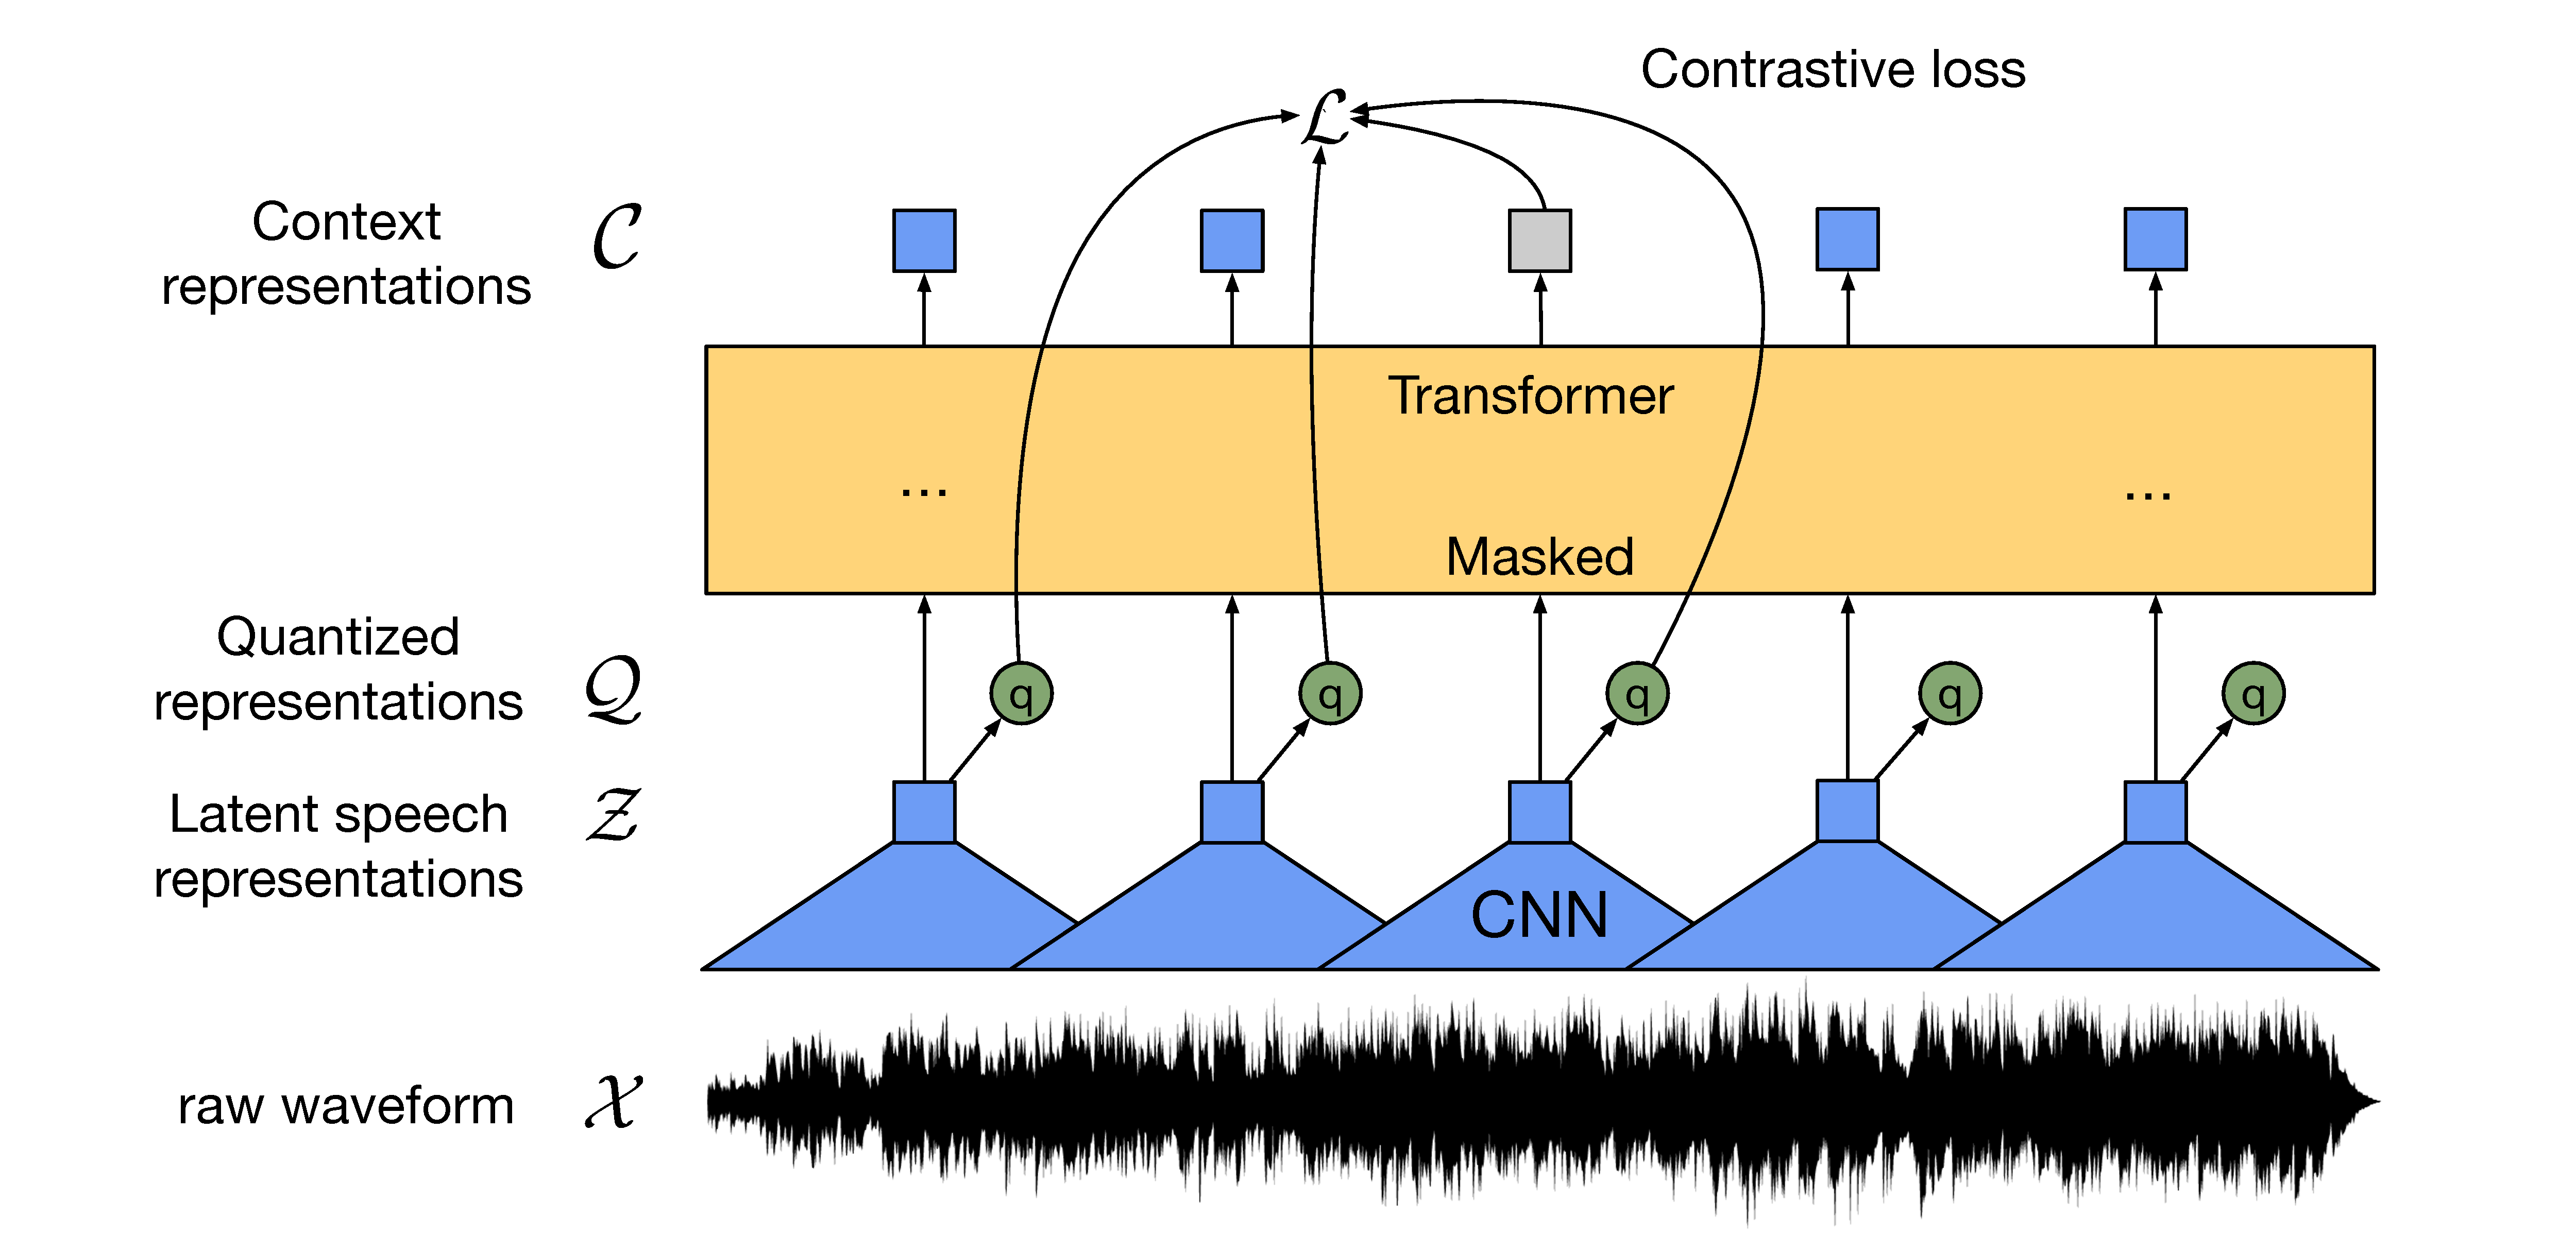
\includegraphics[width=\textwidth]{illustration.pdf}
    \caption{A visualization of the network architecture of wav2vec 2.0, taken from the original paper~\cite{baevski2020wav2vec}.}
    \label{wav2vec2_architecture}
\end{figure}



\subsection{Feature encoder}
The feature encoder maps the raw audio data (speech recordings) to latent speech representations: $f: \mathcal{X} \rightarrow \mathcal{Z}$.
Thus, the feature encoder $f$ maps a sequence of audio samples $\mathbf{x}^{(1)}, \dots \mathbf{x}^{(N)}$ into a sequence of latent feature vectors $\mathbf{z}^{(1)}, \dots, \mathbf{z}^{(t)}$.
% Explain the purpose of feature encoder

The audio data is scaled to have zero mean and unit variance before going into the feature encoder. 
The feature encoder consists of seven convolutional blocks, where each convolutional block contains a temporal\footnote{One-dimensional convolutional layer designed for sequential data.} convolutional layer, 
a layer normalization layer, and the GELU activation function.

Each temporal convolutional layer contains 512 channels. 
The strides of the seven temporal convolutional layers are $(5,2,2,2,2,2,2)$ and the kernel widths are $(10,3,3,3,3,2,2)$.
The strides used results in each $\mathbf{z}^{(t)}$ representing $25$ms of audio (or $400$ input samples),
strided by about $20$ms.

Layer normalization scales the logits after each convolutional layer to have zero mean and unit variance, which has shown to increase the chances of earlier convergence.
GELU has become a popular activation function for NLP related tasks



\subsection{Quantization module}
The quantization module maps the latent speech features into discrete speech units: $h: \mathcal{Z} \rightarrow \mathcal{Q}$.
Speech is sound, and sound is represented as a continuous function. We would like to use Transformers and so continuous representations will not work. 
Unlike written language, which can be discretized into tokens such as characters or sub-words, speech does not have natural sub-units~\cite{bgn2021illustrated}. 
The quantization module is a method in which discrete speech units are automatically learned using product quantization.

To perform product quantization, the quantization module uses $G$ \emph{codebooks}, where each codebook contains $V$ \emph{codebook entries} $\mathbf{e}_{1}, \dots, \mathbf{e}_{V}$.

The following steps describe the process of automatically assigning a discrete speech unit to each latent speech feature $\mathbf{z}^{(t)}$:
\begin{enumerate}
    \item Transform $\mathbf{z}^{(t)}$ into $\mathbf{l}^{(t)} \in \mathbb{R}^{G \times V}$ using a linear transformation.
    \item Choose one codebook entry $\mathbf{e}_g$ for each codebook $g = 1, \dots, G$, based on the values of $\mathbf{l}^{(t)}$.
    \item Concatenate the codebook entries $\mathbf{e}_1, \dots, \mathbf{e}_G$.
    \item Transform the resulting vector into $\mathbf{q}^{(t)} \in \mathbb{R}^{f}$ using another linear transformation.
\end{enumerate}
The two linear transformations are feed-forward neural networks $\text{FF}_1: \mathbb{R}^{f} \rightarrow \mathbb{R}^{G \times V}$ and $\text{FF}_2: \mathbb{R}^{d} \rightarrow \mathbb{R}^{f}$.
In the second step above, the codebook entry $\mathbf{e}_g$ is chosen as the one with the argmax of the logits $\mathbf{l}$. Choosing the codebook entries in this way is non-differentiable.
Fortunately, we can use the Gumbel softmax to choose codebook entries in a fully differentiable way. 
$\mathbf{e}_g$ is chosen as the entry that maximizes
\begin{equation}
    p_{g, v} = \dfrac{\exp{\left(\mathbf{l}^{(t)}_{g, v} + n_v\right)}/\tau}{\sum\limits_{k=1}^{V} \exp{\left(\mathbf{l}^{(t)}_{g, k} + n_k\right)}/\tau},
\end{equation}
where $\tau$ is a non-negative temperature, $n = -\log{(-\log{(u)})}$, and $u$ are uniform samples from $\mathcal{U}(0, 1)$.
During the forward pass, codeword $i$ is chosen by $i = \text{argmax}_j p_{g,j}$ and in the backward pass, the true gradient of the Gumbel softmax outputs is used.



\subsection{Context network}
% Talk about it
The context network, which follows the Transformer architecture, maps the latent speech features into discrete speech units: $h: \mathcal{Z} \rightarrow \mathcal{Q}$.



\subsection{Objective function}
% Talk about it


\section{Connectionist Temporal Classification}
Connectionist Temporal Classification (CTC)~\cite{graves2006connectionist} is an algorithm (or loss function) 
developed to map a sequence of speech features to a sequence of characters. The authors of the wav2vec 2.0 paper
suggest that if finetuning wav2vec 2.0 for ASR one should add a linear layer and CTC on top of the wav2vec 2.0 
network after pretraining on unlabeled audio data.



\subsection{Decoding with CTC}
% TODO: explain with diagram



\subsection{Improving performance with a language model}
% Write about $n$-gram models, Kneser-Nay, and stuff



\section{Finetuning pretrained wav2vec 2.0 models}
% TODO: Make sure what finetuning in my case means EXACTLY (which weights are frozen and which are not).
Pretraining on unlabeled audio data with wav2vec 2.0 is expensive and inconsistent.



\subsection{XLS-R}
% Talk about it
\chapter{EXPERIMENTAL SETUP}

\section{Data sets}

We collected three datasets from which we created the datasets used for pretraining and finetuning. 
Note that the datasets for pretraining and finetuning are mutually exclusive. 
We describe the three datasets in the following paragraphs.

\paragraph*{NCHLT dataset} Majority is used for pre-training, the rest is used for fine-tuning.

\paragraph*{FLEURS dataset} Used for fine-tuning

\paragraph*{High Quality TTS dataset} Used for fine-tuning



\section{Pre-training}

\section{Fine-tuning}

\section{Evaluation metrics}

\paragraph*{Word error rate}
The word error rate (WER) is equal to the number of character-level errors in the predicted transcript, 
divided by the number of words in the true transcript. One character-level error is corrected using one of three operations:
inserting a new character, deleting an existing character, or substituting an existing character for a new character.

\paragraph*{CTC Score/loss} ...
\chapter{RESULTS}
\chapter{CONCLUSIONS}



%%%%%%%%%%%%%%%%%%%%%%%%%%% Bibliography %%%%%%%%%%%%%%%%%%%%%%%%%%%%%%%%%%%%%%%%%%%%%%%%
% \bibliographystyle{usmeg-a} 
\bibliographystyle{unsrt}
\bibliography{biblist}
\addcontentsline{toc}{chapter}{REFERENCES}
\newpage



%%%%%%%%%%%%%%%%%%%%%%%%%%% Insert your appendix here %%%%%%%%%%%%%%%%%%%%%%%%%%%%%%%%%%
\appendix
\begin{appendices}
% \input{Appendices/Questionnaire.tex}
% \input{Appendices/USBStyleSheets.tex}
\end{appendices}


\end{document}